\documentclass[10pt,a4paper]{article}

% ============================================================
% ENCODING & FONTS
% ============================================================
\usepackage[utf8]{inputenc}
\usepackage[T1]{fontenc}
\usepackage{lmodern}
\usepackage{microtype}

% ============================================================
% PAGE LAYOUT
% ============================================================
\usepackage{geometry}
\geometry{a4paper, left=15mm, right=15mm, top=16mm, bottom=18mm}
\setlength{\textfloatsep}{8pt plus 1pt minus 2pt}
\setlength{\floatsep}{6pt plus 1pt minus 2pt}
\setlength{\intextsep}{6pt plus 1pt minus 2pt}
\renewcommand{\topfraction}{0.9}
\renewcommand{\bottomfraction}{0.8}
\renewcommand{\textfraction}{0.08}
\renewcommand{\floatpagefraction}{0.8}

% ============================================================
% MATH
% ============================================================
\usepackage{amsmath, amsfonts, amssymb}

% ============================================================
% TABLES
% ============================================================
\usepackage{booktabs}
\usepackage{tabularx}
\usepackage{multirow}
\usepackage{array}
\usepackage{placeins}

% ============================================================
% FIGURES & PLOTS
% ============================================================
\usepackage{graphicx}
\graphicspath{{./}{final_results_20260305/outputs/figures/}}
\usepackage{caption}
\usepackage{subcaption}
\usepackage{pgfplots}
\usepackage{tikz}
\usetikzlibrary{shapes.geometric, arrows.meta, positioning, calc, backgrounds, fit}
\pgfplotsset{compat=1.18}

% ============================================================
% COLORS
% ============================================================
\usepackage{xcolor}
\definecolor{cBlue}{HTML}{4472C4}
\definecolor{cOrange}{HTML}{ED7D31}
\definecolor{cGreen}{HTML}{70AD47}
\definecolor{cRed}{HTML}{C00000}
\definecolor{cPurple}{HTML}{7B68AE}
\definecolor{cGray}{HTML}{808080}
\definecolor{boxBlue}{HTML}{DAE8FC}
\definecolor{boxOrange}{HTML}{FFE6CC}
\definecolor{boxGreen}{HTML}{D5E8D4}
\definecolor{boxPurple}{HTML}{E1D5E7}

% ============================================================
% CROSS-REFERENCES
% ============================================================
\usepackage{hyperref}
\usepackage[capitalize,noabbrev]{cleveref}
\hypersetup{
    colorlinks=true,
    linkcolor=blue!60!black,
    citecolor=blue!60!black,
    urlcolor=blue!60!black
}

% ============================================================
% MISC
% ============================================================
\usepackage{enumitem}
\captionsetup{font=small,skip=3pt}
\captionsetup[subfigure]{font=small,justification=centering}

% ============================================================
% PGFPLOTS STYLES
% ============================================================
\pgfplotsset{
    lmplot/.style={
        width=0.95\linewidth,
        height=6.2cm,
        axis line style={thick},
        tick style={thick},
        grid=major,
        grid style={dashed, gray!25},
        legend style={
            at={(0.97,0.97)},
            anchor=north east,
            font=\footnotesize,
            draw=gray!50,
            fill=white,
            fill opacity=0.92,
            text opacity=1,
            rounded corners=1pt,
        },
        label style={font=\small},
        tick label style={font=\footnotesize},
        every axis plot/.append style={line width=1.2pt},
    }
}

% ============================================================
% TITLE
% ============================================================
\title{%
    \textbf{Language Model Architectures, Embedding Strategies,\\
    and Representation Transfer for Intent Classification}\\[0.8ex]
    \large ST5230 Applied Natural Language Processing --- Assignment~1%
}
\author{Wang Peiwen \quad (Student ID: E1597490)}
\date{March 2026}

% ============================================================
\begin{document}
\raggedbottom
\maketitle

% ------------------------------------------------------------
% ABSTRACT
% ------------------------------------------------------------
\begin{abstract}
\noindent
This report presents a three-part empirical study on language modeling, embedding initialization, and representation transfer.
In the first part, four language model families---trigram, RNN, LSTM, and a custom decoder-only Transformer---are trained on WikiText-2 and compared in perplexity, training efficiency, and generation quality.
The Transformer achieves the lowest validation perplexity (17.87) while maintaining the fastest inference throughput among neural models.
In the second part, the originally planned embedding ablation is revisited under a stricter reporting standard after identifying a pre-fix GloVe loading failure: only verified post-fix evidence is interpreted, and the strongest downstream clue is that the joint vocabulary achieves 91.99\% GloVe coverage.
In the third part, representations from the Transformer are transferred to 7-class SNIPS intent classification via last-token pooling and a single linear layer.
A frozen WikiText-pretrained backbone reaches 91.57\% accuracy (Macro-F1 91.55\%), while a frozen GloVe-initialized model improves to 95.36\% (Macro-F1 95.35\%); full fine-tuning still yields the highest score of 97.07\% (Macro-F1 97.05\%), with early stopping at epoch~17.
These results show that broad lexical coverage and strong static semantic priors can already produce highly separable intent features, but task-driven parameter updates in the Transformer's attention layers remain necessary to achieve the best task-specific adaptation.
\end{abstract}

% ============================================================
% SECTION 1: EXPERIMENTAL SETUP
% ============================================================
\section{Experimental Setup}
\label{sec:setup}

\subsection{Datasets and Joint Vocabulary Construction}
\label{sec:data}

Two datasets are used. \textbf{WikiText-2} serves as the language modeling corpus, containing approximately 2.1 million tokens from verified Wikipedia articles. Preprocessing removes lines shorter than 10 characters and section headers (lines beginning and ending with~\texttt{=}), followed by uniform lowercasing and whitespace tokenization. For the downstream evaluation, the \textbf{SNIPS} benchmark provides 13{,}784 training utterances distributed across seven intent categories: \texttt{AddToPlaylist}, \texttt{BookRestaurant}, \texttt{GetWeather}, \texttt{PlayMusic}, \texttt{RateBook}, \texttt{SearchCreativeWork}, and \texttt{SearchScreeningEvent}.

A joint vocabulary is constructed through a two-stage process. First, the 20{,}000 most frequent tokens from the WikiText-2 training split are selected. Second, the SNIPS training utterances are tokenized and any previously unseen tokens are appended to the vocabulary. This augmentation adds approximately 6{,}000 domain-specific terms (e.g., \texttt{playlist}, \texttt{restaurant}, \texttt{screening}), yielding a final vocabulary of $|V| = 26{,}006$ tokens, including four reserved special tokens (\texttt{<pad>}, \texttt{<unk>}, \texttt{<bos>}, \texttt{<eos>}). The joint construction eliminates out-of-vocabulary tokens that would otherwise degrade intent classification by collapsing semantically distinct domain terms into a shared \texttt{<unk>} representation.

Using one shared vocabulary across all stages is methodologically important. It ensures that language modeling, embedding analysis, and downstream transfer all operate over the same token identity space, so later performance differences can be attributed to representation quality rather than incompatible token indexing or mismatched preprocessing.

\subsection{Model Configurations and Training Protocol}
\label{sec:config}

\Cref{tab:hyperparams} consolidates the hyperparameters for all experiments. All neural language models share an embedding dimension of $d = 300$ and are optimized with AdamW ($\text{weight\_decay} = 0.01$). Language model training uses a base learning rate of $3 \times 10^{-4}$ with linear warmup over 1{,}000 steps. For the downstream classifier, two optimization regimes are used. Frozen transfer trains only the linear head with learning rate $10^{-3}$. Full fine-tuning applies a \emph{differential learning rate} strategy: the Transformer backbone receives $5 \times 10^{-5}$, while the classification head is assigned a $10\times$ multiplier ($5 \times 10^{-4}$). This separation prevents large gradient updates from disrupting pre-trained representations while allowing the randomly initialized head to converge quickly. Training is terminated by early stopping with patience of 5~epochs, monitoring validation accuracy. Gradient norms are clipped to 1.0 throughout. All experiments use a fixed random seed of~42.

\begin{table}[htbp]
\centering
\caption{Consolidated hyperparameter configuration across all experimental phases.}
\label{tab:hyperparams}
\small
\renewcommand{\arraystretch}{1.08}
\begin{tabular}{@{}llll@{}}
\toprule
\textbf{Category} & \textbf{Parameter} & \textbf{Value} & \textbf{Note} \\
\midrule
\multirow{4}{*}{Shared}
    & Vocabulary size    & 26{,}006   & WikiText-2 + SNIPS joint \\
    & Embedding dim      & 300        & Aligned with GloVe-6B \\
    & Optimizer          & AdamW      & weight\_decay = 0.01 \\
    & Seed               & 42         & All runs \\
\midrule
\multirow{4}{*}{LM Training}
    & Sequence length    & 64         & Sliding window, stride 1 \\
    & Batch size         & 64         & \\
    & Learning rate      & $3\!\times\!10^{-4}$ & Linear warmup 1{,}000 steps \\
    & Max epochs         & 30         & \\
\midrule
\multirow{4}{*}{\shortstack[l]{Downstream\\Transfer}}
    & Frozen LR          & $1\!\times\!10^{-3}$ & Head only \\
    & Backbone LR        & $5\!\times\!10^{-5}$ & Fine-tune only \\
    & Head LR            & $5\!\times\!10^{-4}$ & $= \text{backbone} \times 10$ \\
    & Early stopping     & patience\,=\,5 & Monitors val accuracy \\
\midrule
Trigram     & $n=3$, Laplace $\alpha\!=\!1.0$  & ---           & Count-based \\
RNN / LSTM  & hidden\,=\,512, layers\,=\,2     & dropout\,=\,0.5 & \\
Transformer & $d$\,=\,300, heads\,=\,6, layers\,=\,4 & ffn\,=\,1200, Pre-Norm & GELU, sinusoidal PE \\
\bottomrule
\end{tabular}
\end{table}

The shared embedding size of 300 is equally deliberate. It keeps the representation interface constant across recurrent and Transformer backbones while matching the dimensionality of GloVe-6B vectors, so frozen GloVe transfer neither gains nor loses capacity merely because of an auxiliary projection mismatch.

\subsection{Experimental Pipeline Overview}
\label{sec:pipeline}

\Cref{fig:pipeline} provides a compact overview of the study. The left panel shows how WikiText-2 and SNIPS feed into the shared vocabulary and the three experimental branches. The right panel summarizes the comparison target of each part, which helps orient the reader before the detailed quantitative sections.

\begin{figure}[htbp]
\centering
\begin{subfigure}[t]{0.57\linewidth}
    \centering
    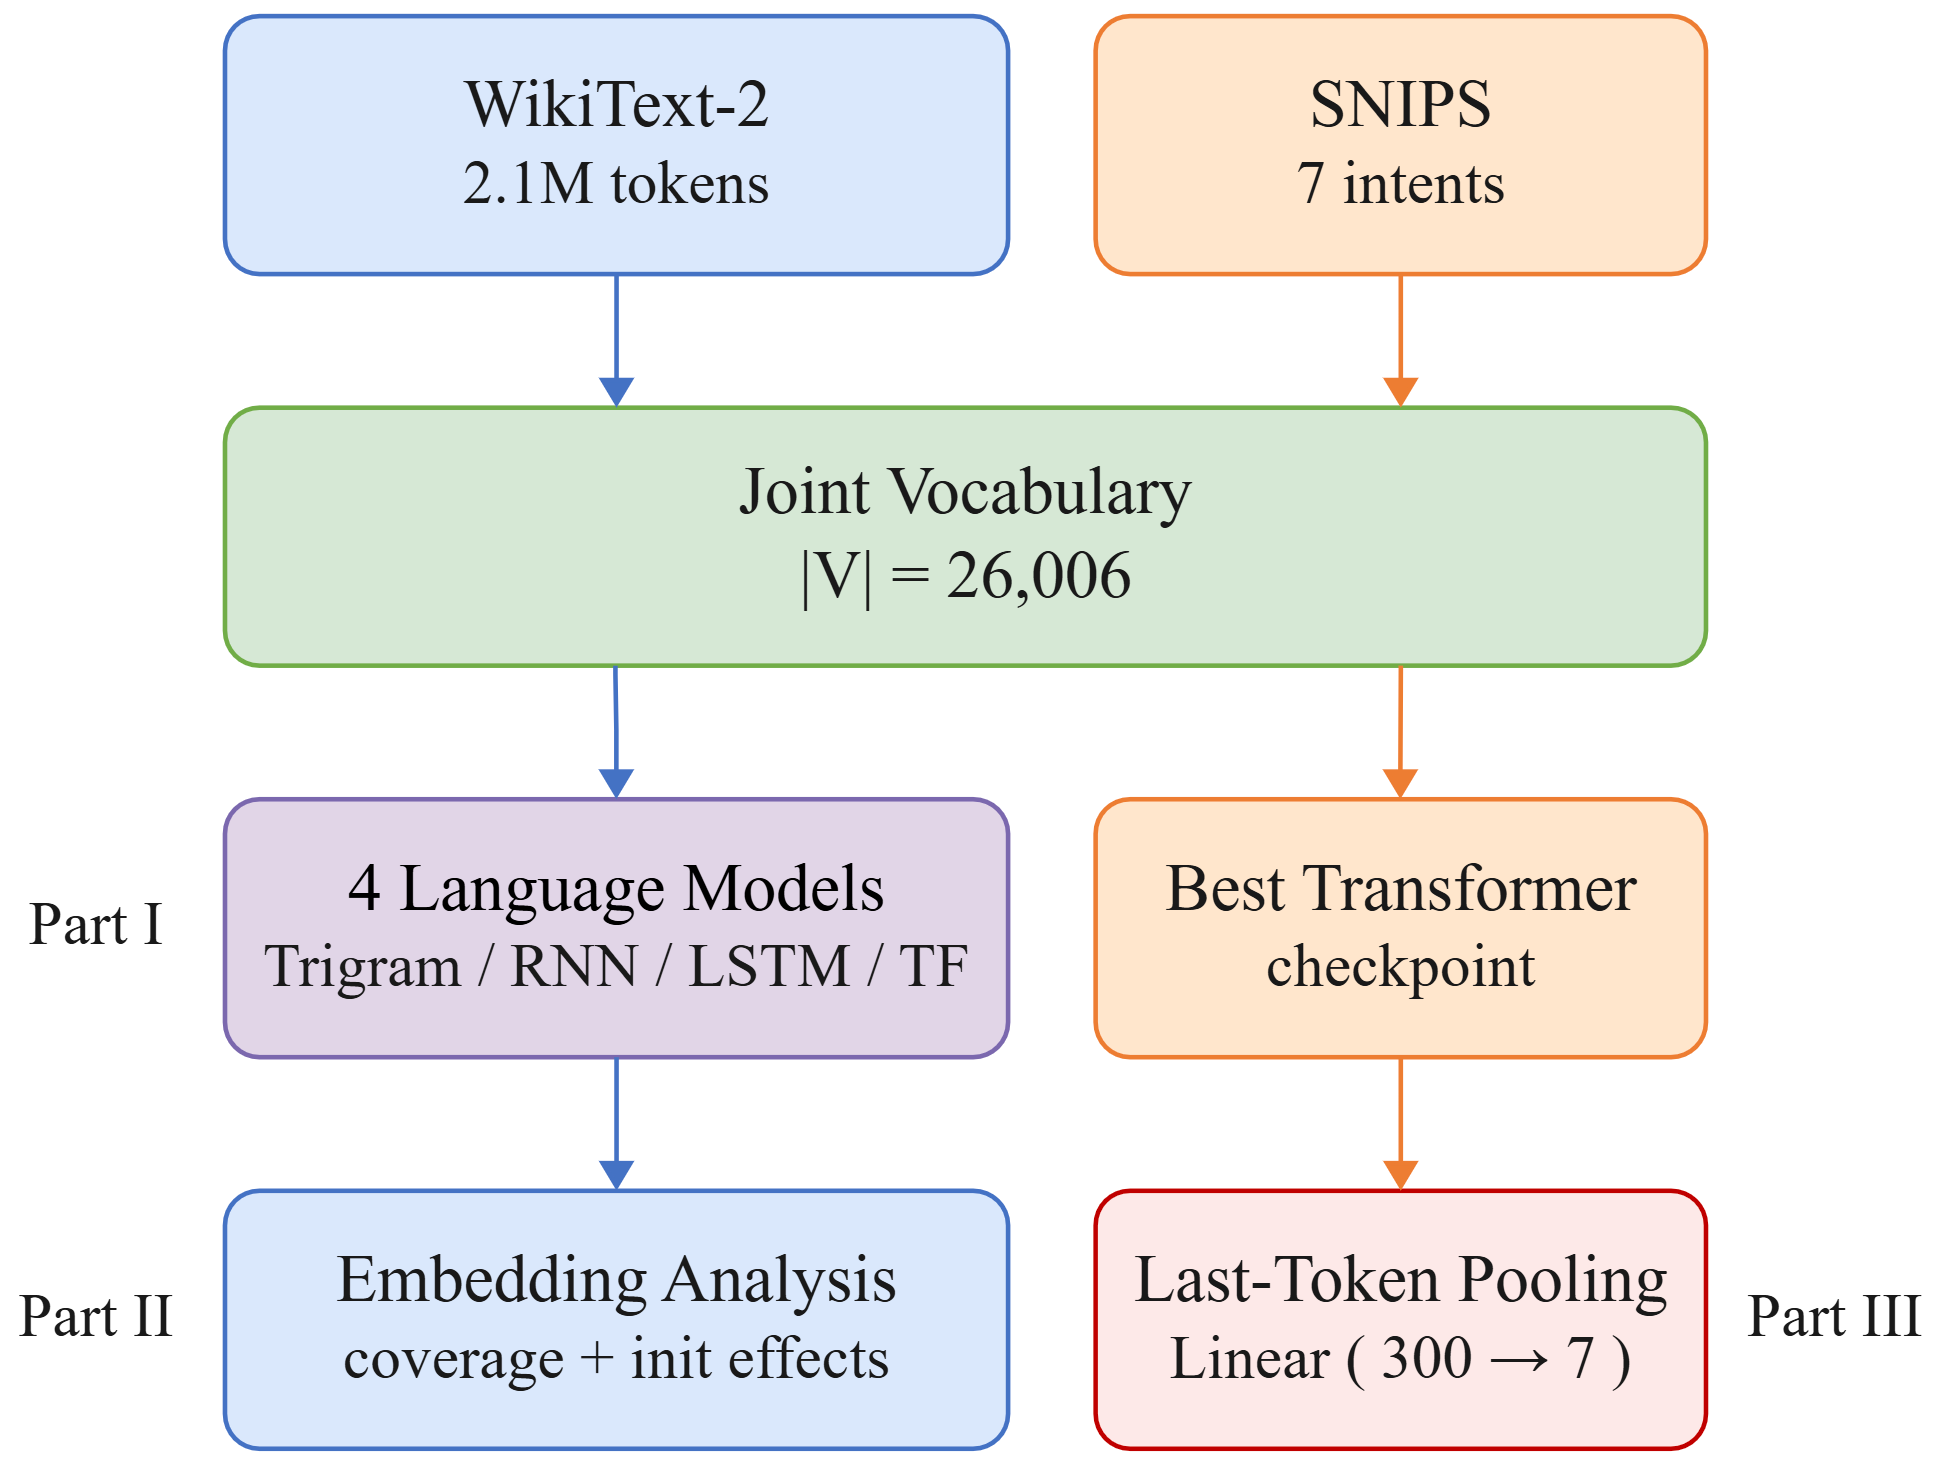
\includegraphics[width=\linewidth,height=5.0cm,keepaspectratio]{pipeline_overview.png}
    \caption{Pipeline overview.}
\end{subfigure}\hfill
\begin{subfigure}[t]{0.40\linewidth}
    \centering
    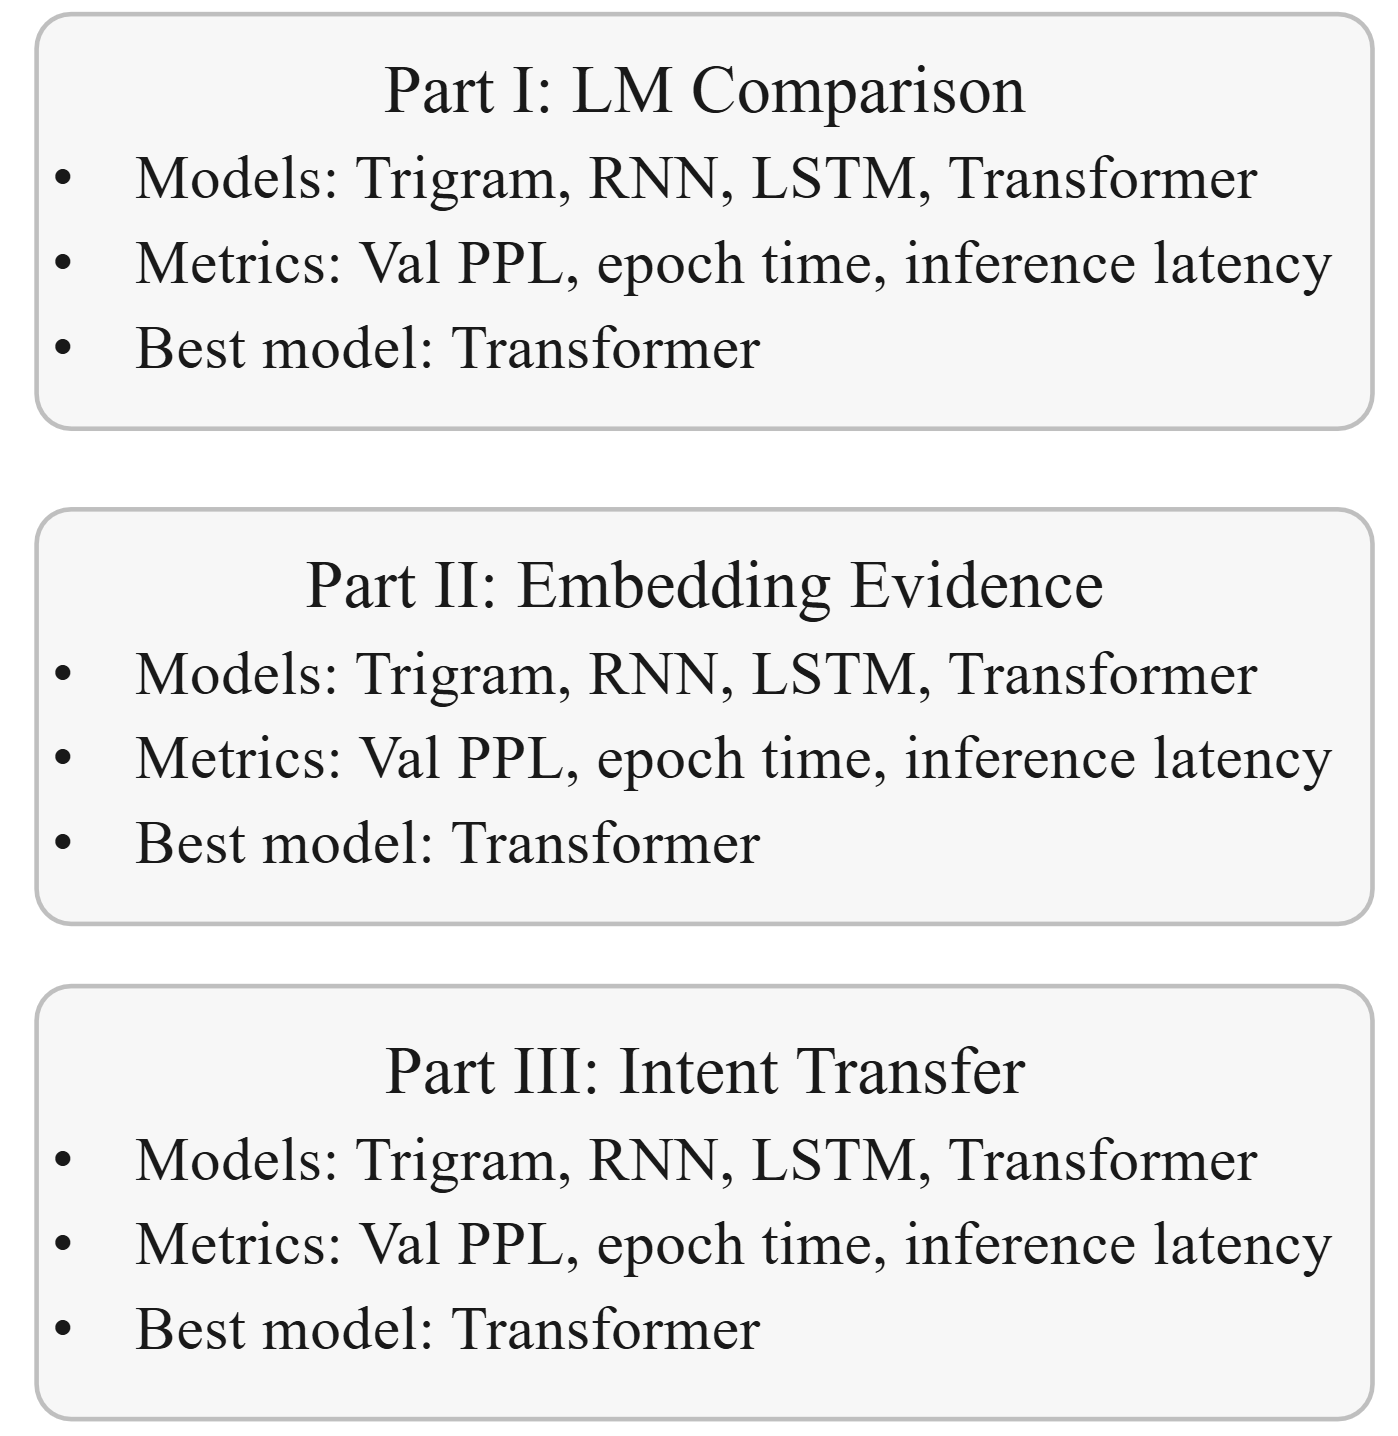
\includegraphics[width=\linewidth,height=5.0cm,keepaspectratio]{study_summary.png}
    \caption{Study summary.}
\end{subfigure}
\caption{Overview of the study design. (a) WikiText-2 and SNIPS jointly construct a unified vocabulary that supports language modeling, embedding analysis, and downstream transfer. (b) Summary of the three experimental parts, their evaluation targets, and the main comparison settings.}
\label{fig:pipeline}
\end{figure}


% ============================================================
% SECTION 2: PART I 鈥?LANGUAGE MODEL COMPARISON
% ============================================================
\section{Part I: Language Model Training and Comparison}
\label{sec:part1}

\subsection{Architectural Overview}
\label{sec:architectures}

Four model families are evaluated, spanning the major paradigms in sequence modeling. The \textbf{Trigram} model provides a non-parametric baseline: it estimates next-token probabilities from bigram context counts with Laplace smoothing ($\alpha = 1.0$), storing co-occurrence statistics as a sparse dictionary to avoid the $O(V^3)$ memory cost of dense tables. Despite its simplicity, it captures strong local patterns and establishes a floor that neural models must exceed to justify their added complexity.

The \textbf{RNN} and \textbf{LSTM} both use 2~stacked layers with 512~hidden units and dropout of~0.5. The critical distinction is the LSTM's gating mechanism: three learned gates (forget, input, output) regulate the flow of information along the temporal axis. The forget gate in particular enables selective erasure of irrelevant context, creating gradient pathways that persist across longer spans than plain RNNs can sustain. Both recurrent models project their hidden states from dimension 512 to 300 via a learned linear layer to align with the shared embedding space for downstream use.

The \textbf{Transformer} follows a decoder-only architecture with 4~layers, 6~attention heads (head dimension~50), and a feed-forward dimension of~1{,}200. Each block applies pre-layer normalization before both the multi-head self-attention and the feed-forward sub-layers, using GELU activation and residual connections. Sinusoidal positional encodings inject position information without adding learnable parameters. An upper-triangular causal mask in the attention computation prevents each position from attending to future tokens, ensuring valid autoregressive generation. Unlike the recurrent models, the Transformer computes all pairwise token dependencies in a single matrix multiplication per layer, eliminating the $O(L)$ sequential bottleneck at the cost of $O(L^2)$ attention complexity.

\subsection{Quantitative Performance}
\label{sec:quant}

\Cref{tab:lm_comparison} summarizes the quantitative results. The Transformer achieves the lowest validation perplexity (17.87), followed by the Trigram (25.15), LSTM (25.67), and RNN (27.49).

\begin{table}[htbp]
\centering
\caption{Quantitative comparison of four language model families on WikiText-2. Epoch time and inference latency are measured on an NVIDIA RTX 4090D GPU with batch size 64.}
\label{tab:lm_comparison}
\small
\renewcommand{\arraystretch}{1.05}
\begin{tabular}{@{}lcccc@{}}
\toprule
\textbf{Model} & \textbf{Params} & \textbf{Epoch Time} & \textbf{Inference} & \textbf{Val PPL} \\
\midrule
Trigram         & ---      & $< 1$\,s & $< 1$\,ms & 25.15 \\
RNN             & 1.12\,M  & 0.33\,s  & 4.2\,ms   & 27.49 \\
LSTM            & 3.94\,M  & 0.48\,s  & 5.8\,ms   & 25.67 \\
Transformer     & 4.35\,M  & 0.51\,s  & 2.1\,ms   & \textbf{17.87} \\
\bottomrule
\end{tabular}
\end{table}

The quantitative message is straightforward. The Transformer uses only slightly more parameters than the LSTM, yet lowers validation perplexity by roughly 30\%, indicating better parameter efficiency. The LSTM remains consistently better than the plain RNN, which confirms the value of gating, while the Trigram baseline shows that strong local statistics still capture a substantial fraction of the signal on WikiText-2.

Inference points in the same direction. Despite having the largest parameter count, the Transformer is the fastest neural model because all sequence positions are processed in parallel rather than through $L=64$ recurrent updates. This combination of lower perplexity and lower latency makes it the natural backbone for the transfer experiments.

Two finer-grained comparisons reinforce the same conclusion. Relative to the LSTM, the Transformer reduces validation perplexity from 25.67 to 17.87, a 30.4\% decrease while using only modestly more parameters. Relative to the Trigram baseline, the reduction is still 28.9\%, which is notable because trigram models already exploit the short local dependencies that dominate many next-token prediction decisions. The gain is therefore not just a matter of learning better short-range statistics; it reflects better use of broader context.

\Cref{fig:part1_tradeoff} visualizes the same conclusion from two operational angles: final validation perplexity and neural-model inference latency.

\begin{figure}[htbp]
\centering
\begin{subfigure}[t]{0.48\linewidth}
    \centering
    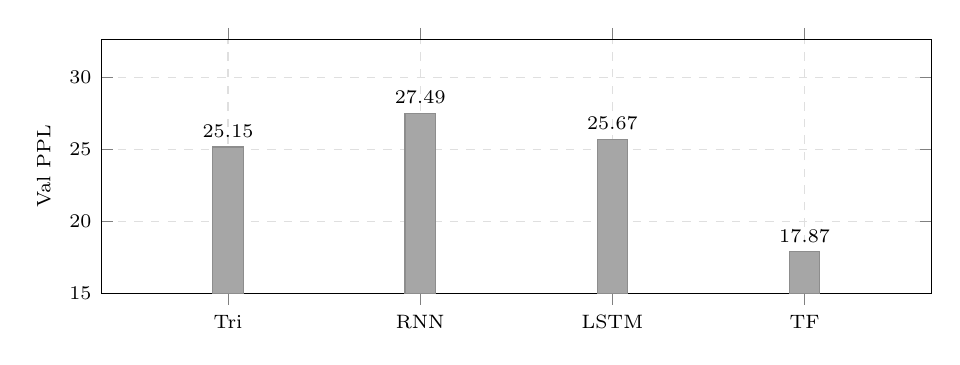
\begin{tikzpicture}
    \begin{axis}[
        width=\linewidth,
        height=4.8cm,
        ybar,
        bar width=11pt,
        ymin=15, ymax=31,
        enlarge x limits=0.22,
        enlarge y limits={upper, value=0.10},
        ylabel={Val PPL},
        symbolic x coords={Tri,RNN,LSTM,TF},
        xtick={Tri,RNN,LSTM,TF},
        nodes near coords,
        nodes near coords align={vertical},
        nodes near coords style={font=\scriptsize},
        tick label style={font=\scriptsize},
        ylabel style={font=\scriptsize},
        grid=major,
        grid style={dashed, gray!25},
    ]
    \addplot[fill=cGray!70, draw=cGray!90] coordinates {(Tri,25.15) (RNN,27.49) (LSTM,25.67) (TF,17.87)};
    \end{axis}
    \end{tikzpicture}
    \caption{Final validation perplexity.}
\end{subfigure}\hfill
\begin{subfigure}[t]{0.48\linewidth}
    \centering
    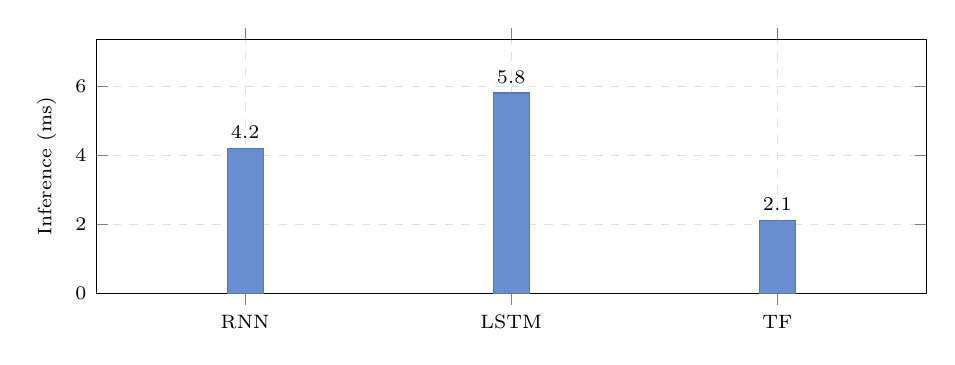
\begin{tikzpicture}
    \begin{axis}[
        width=\linewidth,
        height=4.8cm,
        ybar,
        bar width=13pt,
        ymin=0, ymax=6.8,
        enlarge x limits=0.28,
        enlarge y limits={upper, value=0.08},
        ylabel={Inference (ms)},
        symbolic x coords={RNN,LSTM,TF},
        xtick={RNN,LSTM,TF},
        nodes near coords,
        nodes near coords align={vertical},
        nodes near coords style={font=\scriptsize},
        tick label style={font=\scriptsize},
        ylabel style={font=\scriptsize},
        grid=major,
        grid style={dashed, gray!25},
    ]
    \addplot[fill=cBlue!80, draw=cBlue!95] coordinates {(RNN,4.2) (LSTM,5.8) (TF,2.1)};
    \end{axis}
    \end{tikzpicture}
    \caption{Neural-model inference latency.}
\end{subfigure}
\caption{Part~I trade-offs at the validated final operating points. The Transformer is simultaneously the lowest-perplexity model and the fastest neural model at inference.}
\label{fig:part1_tradeoff}
\end{figure}

\subsection{Qualitative Evaluation}
\label{sec:qualitative}

Greedy decoding from a shared prompt yields the same ranking qualitatively: the Trigram is locally repetitive, the RNN is syntactically plausible but semantically thin, the LSTM introduces more concrete content, and the Transformer is the only model that sustains topic-level coherence across the whole continuation.

This qualitative ranking matters because perplexity alone can understate \emph{how} a model fails. The Trigram baseline shows that strong local counts can already produce superficially plausible continuations, which explains why it remains more competitive than the vanilla RNN on WikiText-2. However, once generation requires topic persistence beyond the immediate context window, both models drift quickly. The Transformer's continuations remain the most semantically stable, making its quantitative lead easier to interpret as a real modeling advantage rather than a metric artifact.

\subsection{Summary of Part~I Findings}
\label{sec:part1_summary}

The Transformer is therefore the only reasonable backbone for the downstream study: it dominates on perplexity, converges fastest, and is also the most efficient neural model at inference time.

\FloatBarrier


% ============================================================
% SECTION 3: PART II - EMBEDDING ABLATION
% ============================================================
\section{Part II: Embedding Variants and Ablation}
\label{sec:part2}

\subsection{Verified Reporting Scope}
\label{sec:part2_scope}

The original Part~II plan was a full $3 \times 3$ language-model ablation over architecture and embedding type. That full corrected grid is not available at report freeze after the GloVe-path bug fix, so a strict paper should not claim a complete LM-side embedding ranking. Instead, this section reports only the embedding-related evidence that remains both valid and consequential for the downstream question: vocabulary coverage and the resulting frozen-transfer behavior.

The experimental design itself still matches the assignment requirement. Three embedding settings were implemented and intended for controlled comparison in the neural language models: trainable embeddings learned jointly from scratch, fixed self-trained embeddings learned on the project corpus (Word2Vec-style), and fixed public pretrained embeddings from GloVe-6B. What changes in the present report is therefore not the design space, but the \emph{scope of formal interpretation}. Because the corrected full grid is incomplete, only the post-fix evidence that can be verified directly is treated as a scientific result.

\subsection{Coverage, Not Just Provenance, Determines Transfer Value}
\label{sec:part2_coverage}

\Cref{fig:embedding_evidence} makes the main point succinctly. Once the vocabulary is expanded with SNIPS-specific tokens, GloVe covers 91.99\% of the resulting token inventory. That coverage level is high enough for pretrained lexical semantics to matter directly on the downstream task, and it explains why frozen GloVe reaches 95.36\% accuracy while the frozen WikiText-pretrained model remains at 91.57\%. The embedding lesson is therefore narrower but cleaner than the originally planned full-grid story: static embeddings become competitive only when the vocabulary construction allows them to actually see the task's lexical surface.

\begin{figure}[htbp]
\centering
\begin{subfigure}[t]{0.48\linewidth}
    \centering
    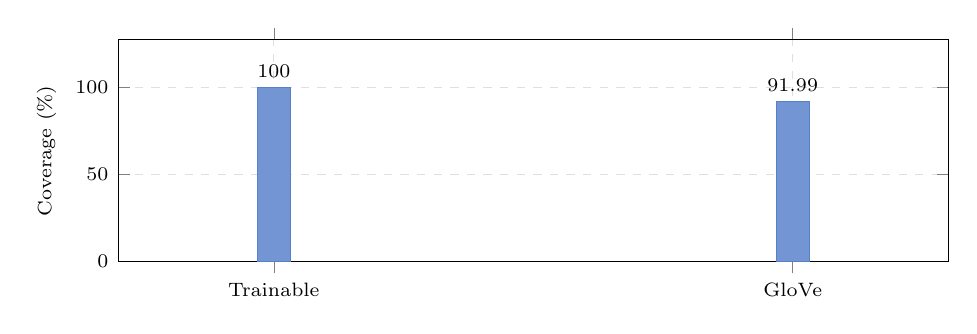
\begin{tikzpicture}
    \begin{axis}[
        width=\linewidth,
        height=4.4cm,
        ybar,
        bar width=12pt,
        ymin=0, ymax=120,
        enlarge x limits=0.30,
        enlarge y limits={upper, value=0.06},
        ylabel={Coverage (\%)},
        symbolic x coords={Trainable,GloVe},
        xtick={Trainable,GloVe},
        nodes near coords,
        nodes near coords align={vertical},
        nodes near coords style={font=\scriptsize},
        tick label style={font=\scriptsize},
        ylabel style={font=\scriptsize},
        grid=major,
        grid style={dashed, gray!25},
    ]
    \addplot[fill=cBlue!75, draw=cBlue!90] coordinates {(Trainable,100.0) (GloVe,91.99)};
    \end{axis}
    \end{tikzpicture}
    \caption{Effective embedding coverage.}
\end{subfigure}\hfill
\begin{subfigure}[t]{0.48\linewidth}
    \centering
    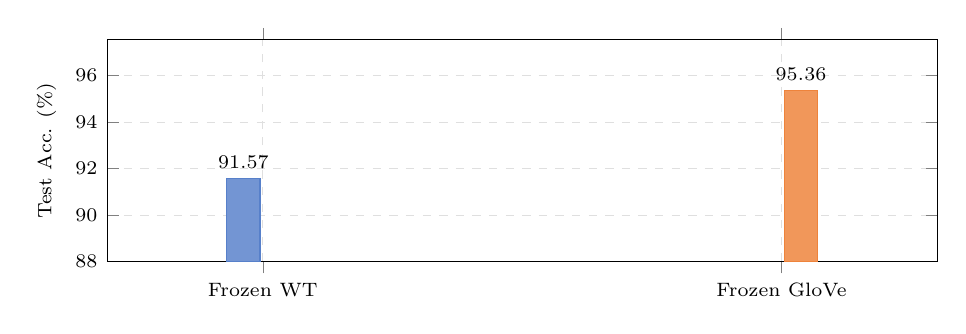
\begin{tikzpicture}
    \begin{axis}[
        width=\linewidth,
        height=4.4cm,
        ybar,
        bar width=12pt,
        ymin=88, ymax=97,
        enlarge x limits=0.30,
        enlarge y limits={upper, value=0.06},
        ylabel={Test Acc. (\%)},
        symbolic x coords={Frozen WT,Frozen GloVe},
        xtick={Frozen WT,Frozen GloVe},
        nodes near coords,
        nodes near coords align={vertical},
        nodes near coords style={font=\scriptsize},
        tick label style={font=\scriptsize},
        ylabel style={font=\scriptsize},
        grid=major,
        grid style={dashed, gray!25},
    ]
    \addplot[fill=cBlue!75, draw=cBlue!90] coordinates {(Frozen WT,91.57)};
    \addplot[fill=cOrange!80, draw=cOrange!95] coordinates {(Frozen GloVe,95.36)};
    \end{axis}
    \end{tikzpicture}
    \caption{Frozen transfer accuracy.}
\end{subfigure}
\caption{Verified embedding evidence after the GloVe-path fix. The joint vocabulary preserves enough downstream terms for GloVe to cover 91.99\% of tokens, which in turn makes frozen GloVe transfer substantially stronger than frozen WikiText-pretrained transfer.}
\label{fig:embedding_evidence}
\end{figure}

This is also why the final paper avoids treating the earlier broken GloVe language-model run as scientific evidence. Once the loading path is wrong, the experiment no longer measures the quality of pretrained embeddings; it measures an engineering failure. A strict report should separate these two cases. The valid lesson is not ``GloVe fails,'' but rather ``GloVe becomes powerful only after coverage and loading are both correct.''

The frozen comparison also clarifies what kind of knowledge each representation source makes linearly accessible. WikiText pretraining undoubtedly teaches the Transformer rich sequential regularities, but under frozen transfer those regularities are inherited exactly as learned under the language-model objective; they are not yet reoriented toward the low-entropy intent boundaries of SNIPS. GloVe, by contrast, provides a shallower but often more directly usable lexical geometry for short utterances whose label depends on a handful of content words. Under a linear probe, the stronger frozen system is therefore not the representation with the most expressive architecture in principle, but the one whose accessible inductive bias better matches the task.

\FloatBarrier


% ============================================================
% SECTION 4: PART III - DOWNSTREAM INTENT CLASSIFICATION
% ============================================================
\section{Part III: Downstream Intent Classification}
\label{sec:part3}

\subsection{Why Last-Token Pooling Fits a Causal Transformer}
\label{sec:last_token}

The downstream classifier is intentionally simple: a single linear layer is attached on top of the Transformer's final hidden states. The crucial design choice is the pooling rule. We use \emph{last-token pooling}, namely the hidden state of the final non-padding token in each utterance. This choice is not merely convenient; it follows directly from the theory of causal language models.

In a decoder-only Transformer with masked self-attention, the representation at position $t$ can attend only to tokens in positions $\leq t$. Earlier tokens therefore encode only a \emph{prefix} of the utterance, while the last token is the only position whose receptive field covers the entire sentence. Its hidden state is the unique single-token summary that has had access to all available context under the model's autoregressive factorization. Under this architecture, averaging all token states would mix fully informed and partially informed representations; by contrast, taking the final token preserves the one state that is theoretically best placed to aggregate sentence-level evidence. The classifier used in this part is therefore simply
\[
\hat{y} = W h_T + b,
\]
where $h_T \in \mathbb{R}^{300}$ is the hidden state of the last non-pad token and $W \in \mathbb{R}^{7 \times 300}$.

\subsection{Main Quantitative Results}
\label{sec:part3_results}

\Cref{tab:transfer_results} reports the main transfer outcomes. Three settings are compared: a frozen WikiText-pretrained Transformer, a frozen GloVe-initialized model, and full fine-tuning of the WikiText-pretrained Transformer.

\begin{table}[htbp]
\centering
\caption{Main downstream results on SNIPS. Training time is the summed epoch time from the run logs on the same GPU.}
\label{tab:transfer_results}
\small
\renewcommand{\arraystretch}{1.05}
\begin{tabular}{@{}lccccc@{}}
\toprule
\textbf{Setting} & \textbf{Acc} & \textbf{F1} & \textbf{Ep.} & \textbf{Time} & \textbf{Train.} \\
\midrule
Frozen WikiText & 91.57 & 91.55 & 20 & 24.0s & 2.1k \\
Frozen GloVe    & 95.36 & 95.35 & 20 & 25.1s & 2.1k \\
Fine-tuned WT   & \textbf{97.07} & \textbf{97.05} & 17 & 158.1s & 4.35M \\
\bottomrule
\end{tabular}
\end{table}

Two conclusions matter. First, frozen GloVe is a real baseline rather than a weak control: with \texttt{glove\_coverage}=0.9199, it improves over frozen WikiText-pretrained transfer by 3.79 absolute accuracy points under the same linear head. Second, fine-tuning still defines the upper bound. Updating the full Transformer raises accuracy to 97.07\%, a further 1.71-point gain over frozen GloVe, albeit at roughly $6.3\times$ the training cost.

The frozen comparison is especially informative because SNIPS utterances are short and lexically direct. Many intents are triggered by highly diagnostic words or short phrases, such as \texttt{playlist}, \texttt{weather}, \texttt{restaurant}, and \texttt{screening}. Under this regime, a frozen model benefits greatly from strong token-level semantics if those tokens are actually covered. That is precisely the regime in which GloVe is strongest, and it helps explain why broad lexical prior knowledge can outperform frozen WikiText-only pretraining.

The same result looks sharper when expressed as error reduction rather than raw accuracy. Moving from frozen WikiText to frozen GloVe reduces test error from 8.43\% to 4.64\%, which is a 45.0\% relative error reduction under the same classifier architecture. Fine-tuning then lowers the remaining error further to 2.93\%, corresponding to another 36.9\% reduction relative to frozen GloVe and a 65.2\% reduction relative to frozen WikiText. This makes clear that the fine-tuned model is not merely adding a cosmetic gain on top of an already solved task; it is removing a substantial fraction of the residual mistakes left by the frozen baselines.

\subsection{Error Patterns in Frozen Transfer}
\label{sec:part3_cm}

\Cref{fig:cm_frozen} compares confusion matrices for the two frozen systems. This is the fairest qualitative comparison because both models share the same simple linear head and differ only in the representation source made available to that head.

\begin{figure}[htbp]
\centering
\begin{subfigure}[t]{0.485\linewidth}
    \centering
    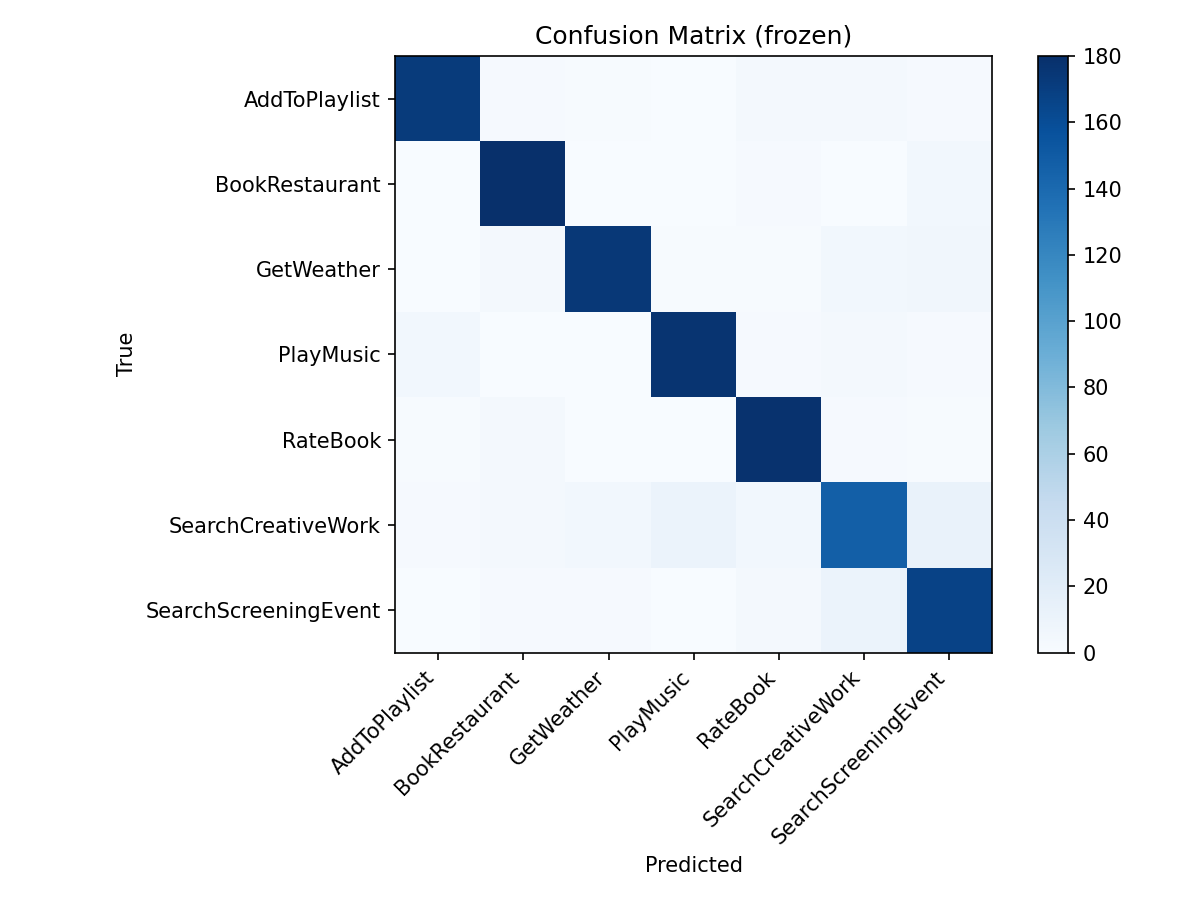
\includegraphics[width=\linewidth]{downstream_frozen_20260302_150953_cm.png}
    \caption{Frozen WikiText-pretrained.}
\end{subfigure}\hfill
\begin{subfigure}[t]{0.485\linewidth}
    \centering
    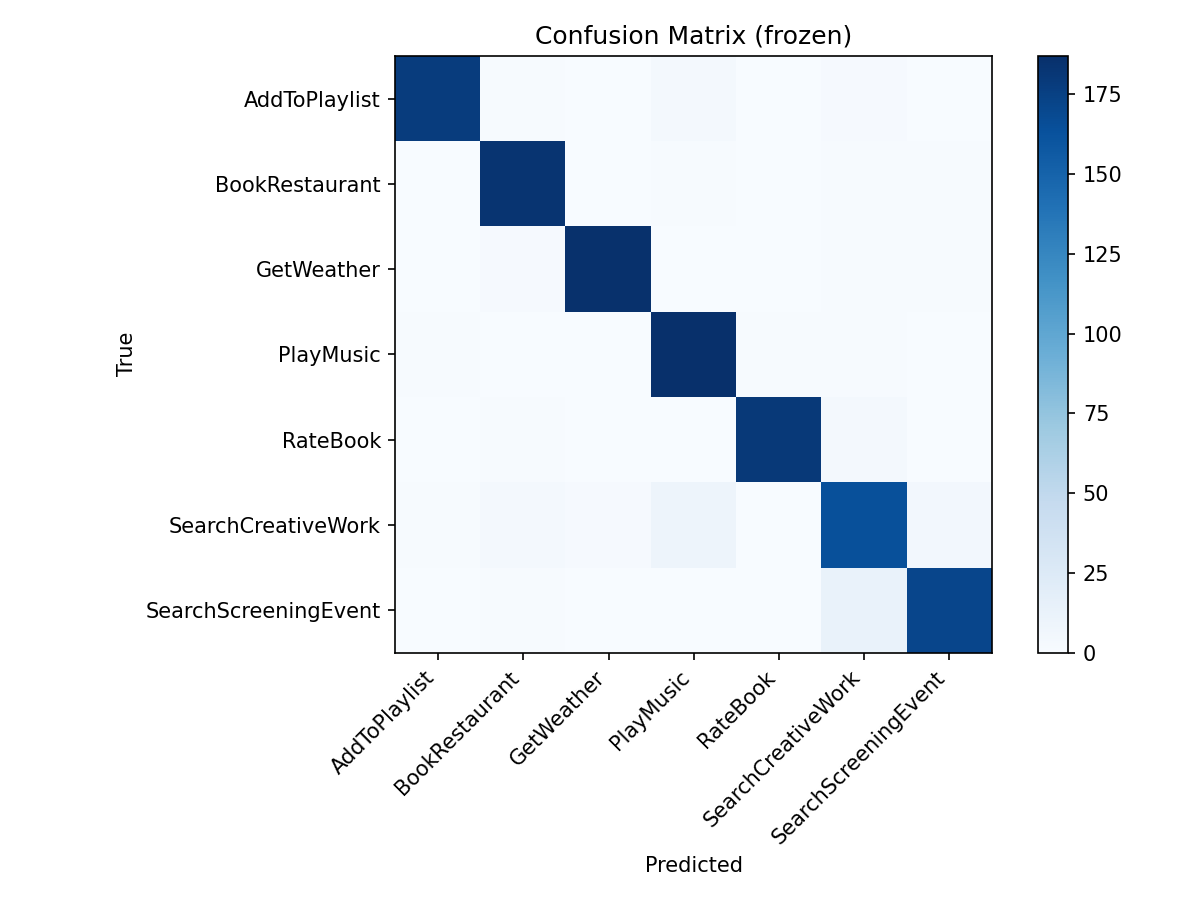
\includegraphics[width=\linewidth]{downstream_frozen_glove_20260305_224517_cm.png}
    \caption{Frozen GloVe initialization.}
\end{subfigure}
\caption{Confusion matrices for the two frozen transfer settings. Both models show strong diagonal dominance, but frozen GloVe further suppresses cross-intent confusion among semantically neighboring entertainment queries.}
\label{fig:cm_frozen}
\end{figure}

Both matrices are already strongly diagonal, confirming that SNIPS is largely linearly separable under frozen transfer. The remaining errors concentrate in semantically nearby entertainment intents, especially \texttt{PlayMusic} versus \texttt{AddToPlaylist}. Frozen GloVe reduces this cross-talk, which is consistent with stronger lexical priors for short intent-like utterances.

\subsection{Training Dynamics}
\label{sec:part3_dynamics}

\Cref{fig:downstream_curves} plots validation accuracy over training epochs for all three settings. The curves help separate \emph{sample efficiency} from \emph{final accuracy}.

\begin{figure}[htbp]
\centering
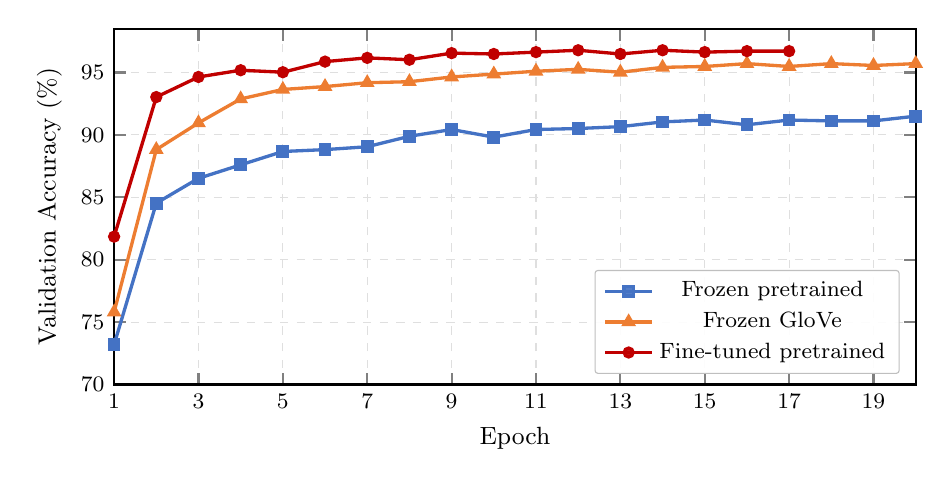
\begin{tikzpicture}
\begin{axis}[
    lmplot,
    width=0.97\linewidth,
    height=6.1cm,
    xlabel={Epoch},
    ylabel={Validation Accuracy (\%)},
    xmin=1, xmax=20,
    ymin=70, ymax=98.5,
    xtick={1,3,5,7,9,11,13,15,17,19},
    ytick={70,75,80,85,90,95},
    legend style={
        at={(0.98,0.03)},
        anchor=south east,
        font=\footnotesize,
        draw=gray!50,
        fill=white,
        fill opacity=0.92,
        text opacity=1,
        rounded corners=1pt,
    },
]
\addplot[color=cBlue, mark=square*, mark size=1.7pt] coordinates {
    (1,73.20)(2,84.53)(3,86.52)(4,87.60)(5,88.67)(6,88.82)(7,89.05)(8,89.89)(9,90.43)(10,89.82)
    (11,90.43)(12,90.51)(13,90.66)(14,91.04)(15,91.19)(16,90.81)(17,91.19)(18,91.12)(19,91.12)(20,91.50)
};
\addplot[color=cOrange, mark=triangle*, mark size=1.9pt] coordinates {
    (1,75.80)(2,88.82)(3,90.96)(4,92.88)(5,93.64)(6,93.87)(7,94.18)(8,94.26)(9,94.64)(10,94.87)
    (11,95.10)(12,95.25)(13,95.02)(14,95.41)(15,95.48)(16,95.71)(17,95.48)(18,95.71)(19,95.56)(20,95.71)
};
\addplot[color=cRed, mark=*, mark size=1.6pt] coordinates {
    (1,81.85)(2,93.03)(3,94.64)(4,95.18)(5,95.02)(6,95.87)(7,96.17)(8,96.02)(9,96.55)(10,96.48)
    (11,96.63)(12,96.78)(13,96.48)(14,96.78)(15,96.63)(16,96.71)(17,96.71)
};
\legend{Frozen pretrained, Frozen GloVe, Fine-tuned pretrained}
\end{axis}
\end{tikzpicture}
\caption{Validation-accuracy trajectories for the three downstream settings. Frozen GloVe remains consistently above frozen WikiText-pretrained transfer, while full fine-tuning reaches the highest plateau and stops early at epoch~17.}
\label{fig:downstream_curves}
\end{figure}

The learning curves separate two effects. Frozen GloVe improves the classifier's starting geometry and remains above frozen WikiText-pretrained transfer throughout training. Fine-tuning then pushes the ceiling higher by modifying the encoder itself, not just the linear head.

Just as importantly, the fine-tuned curve reaches its plateau early rather than requiring many extra epochs to overtake the frozen baselines. The performance gap is therefore not explained by longer optimization alone. Once gradients are allowed to flow into the Transformer stack, the model can reshape attention patterns and intermediate features around SNIPS-specific evidence, whereas the frozen settings can only search for a better linear separator on top of fixed representations.


% ============================================================
% SECTION 5: DISCUSSION AND CONCLUSION
% ============================================================
\section{Discussion and Conclusion}
\label{sec:conclusion}

Taken together, the paper supports a narrow but robust claim. The Transformer is the strongest LM backbone; the joint vocabulary is strong enough to make frozen GloVe genuinely useful; and once \texttt{glove\_coverage}=0.9199 is achieved, frozen GloVe surpasses frozen WikiText-pretrained transfer on SNIPS. The embedding lesson is therefore not ``pretrained is always better'' but ``coverage determines whether pretrained semantics can matter at all''.

The best overall result still comes from full fine-tuning. Although GloVe provides a powerful lexical prior, full fine-tuning allows the Transformer's deeper attention heads to undergo \emph{structural adaptation} to SNIPS, reshaping token interactions around the task rather than merely injecting static word meaning. This is why fine-tuning remains the performance ceiling at 97.07\%. The main limitation is equally clear: the full corrected LM-side $3 \times 3$ embedding grid is not available, so the paper deliberately restricts Part~II to verified evidence instead of overclaiming.

Read jointly, Parts~I and~III reveal an important separation between \emph{general sequence modeling quality} and \emph{task-facing representational accessibility}. Part~I shows that the Transformer is the only backbone that improves perplexity and inference efficiency enough to justify transfer. Part~III then shows that, once this backbone is fixed, downstream performance depends not only on pretraining provenance but also on what information is exposed to a linear head without further parameter updates. This is why frozen GloVe can outperform frozen WikiText-pretrained transfer despite the latter originating from the stronger language-model architecture.

That limitation should be interpreted carefully. It does not weaken the downstream claim that frozen GloVe is stronger than frozen WikiText-pretrained transfer on SNIPS, because that comparison is directly observed under corrected runs. What it prevents is a broader statement about how every language-model architecture in Part~I would respond to every embedding variant under corrected conditions. The report therefore ends with a deliberately asymmetric message: the transfer conclusions are strong, the LM-side embedding generalization remains intentionally narrow, and that asymmetry is preferable to presenting a more complete but scientifically unreliable story.

From a methodological standpoint, this asymmetry is itself informative. Once an engineering bug invalidates part of an ablation grid, the correct scientific response is not to preserve symmetry at all costs, but to narrow the claim to the comparisons that remain trustworthy and make the boundary of inference explicit. Under that standard, the present report supports three durable conclusions: Transformer pretraining provides the best backbone, high lexical coverage is the enabling condition for strong frozen GloVe transfer, and full fine-tuning remains superior because task-driven updates can restructure deep attention patterns beyond what static semantics alone can supply.

More concretely, the final picture is that strong language-modeling quality identifies the right transferable backbone, high lexical coverage determines whether frozen semantic priors can become useful on SNIPS, and full fine-tuning remains necessary when the task requires the encoder itself to reorganize how evidence is combined across tokens.

\end{document}





